% gc-05-TrigDiff.tex

\documentclass[xcolor=dvipsnames]{beamer}
\usepackage{teachbeamer}

\title{Differentiating Trigonometric Functions}
\subtitle{{\CourseNumber}, BCIT}

\author{\CourseName}

\date{January 22, 2018}

% \begin{figure}[h]
% 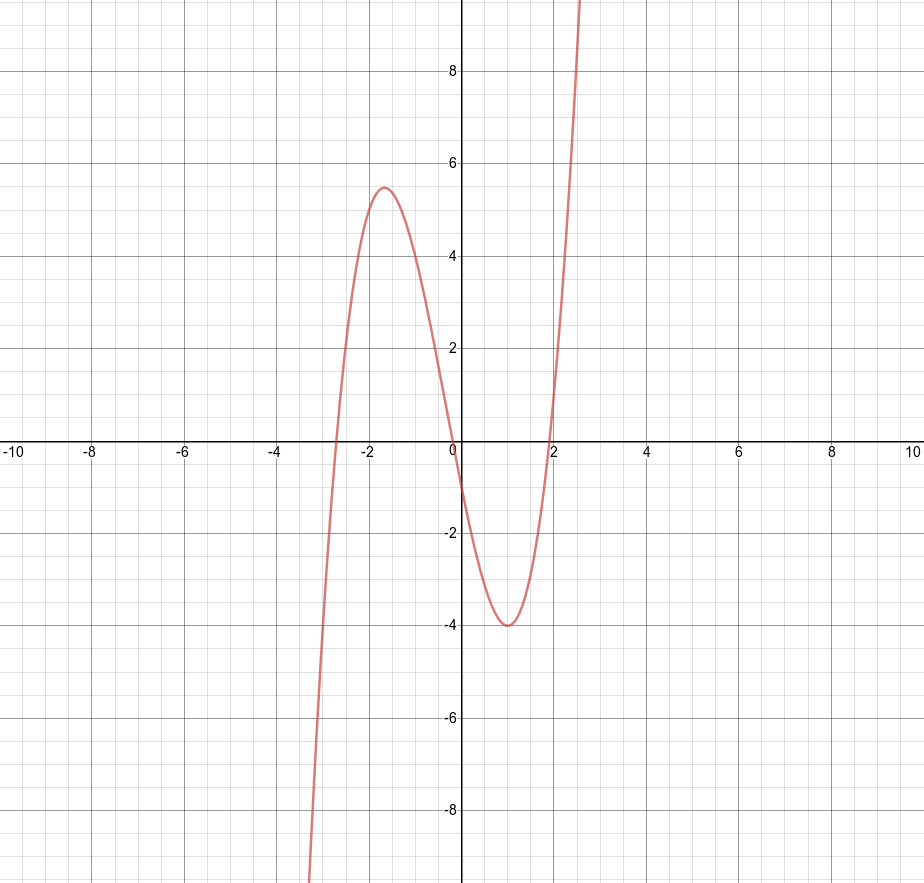
\includegraphics[scale=.3]{./diagrams/extrema1.png}
% \end{figure}

\begin{document}

\begin{frame}
  \titlepage
\end{frame}

\begin{frame}
  \frametitle{Trigonometric Functions Review}
Make sure to remember that the trigonometric functions (sine, cosine,
tangent, cotangent, etc.) are functions from the real numbers into the
real numbers. An angle is a real number in terms of its
\alert{radians} measure. If the angle is in degrees, it can be
converted to radians as in the following example,
\begin{equation}
  \label{eq:eedeehuc}
  42^{\circ}=42\cdot\frac{\pi}{180}\approx{}0.73304
\end{equation}
% The derivative of $f(\vartheta)=\sin\vartheta$ is 
% \begin{equation}
%   \label{eq:eishooro}
%   f'(\vartheta)=\cos\vartheta
% \end{equation}
% For a proof, see James Stewart, \emph{Single Variable Calculus}, Sixth
% Edition, page 190f (or page 135). 
% \emph{Exercise:} Differentiate $f(x)=x^{2}\sin{}x$.
\end{frame}

\begin{frame}
  \frametitle{Trigonometric Functions Review}
  This reference triangle serves as a reminder how the sine and cosine
  are defined. Any right triangle whose hypotenuse is of length $c'=1$
  can be inserted into the unit circle so that one of the two shorter
  sides rests on the $x$-axis and one of the vertices is at the
  origin. Then the vertex $B$ in the diagram has the coordinates
  $(\cos\alpha,\sin\alpha)$.
    \begin{figure}[h]
    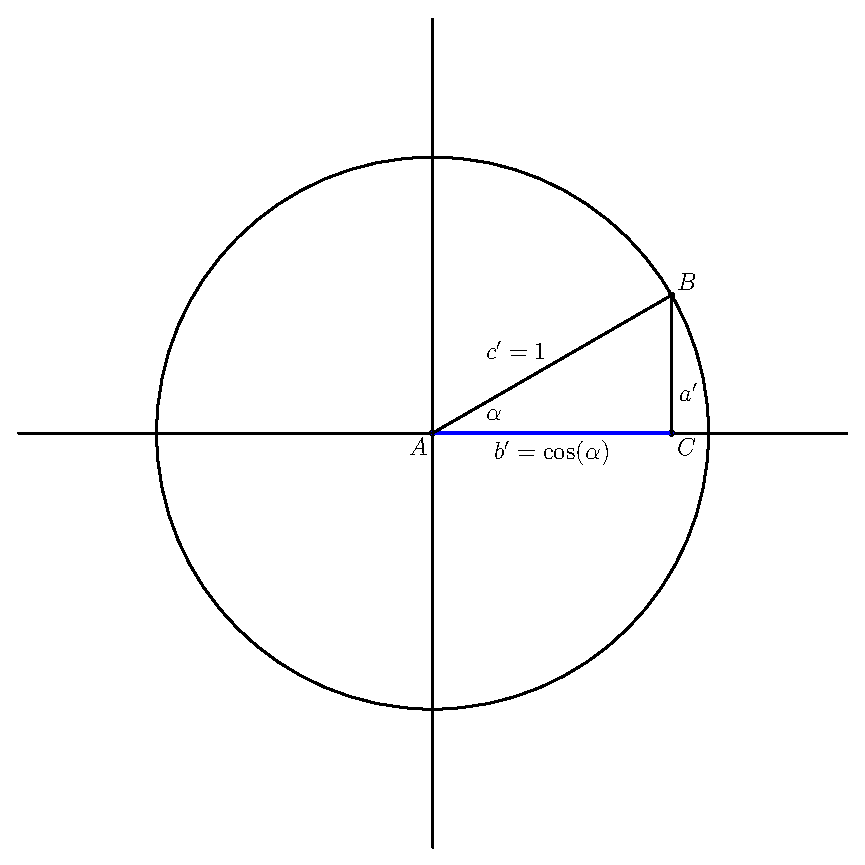
\includegraphics[scale=.5]{./diagrams/cosine.eps}
  \end{figure}
\end{frame}

\begin{frame}
  \frametitle{Trigonometric Functions Review}
  The remaining trigonometric functions are defined as follows.
  \begin{equation}
    \label{eq:eiyiexir}
    \tan{}x=\frac{\sin{}x}{\cos{}x}
  \end{equation}
  \begin{equation}
    \label{eq:dohquohb}
    \cot{}x=\frac{\cos{}x}{\sin{}x}=\frac{1}{\tan{}x}
  \end{equation}
  \begin{equation}
    \label{eq:eengohqu}
    \csc{}x=\frac{1}{\sin{}x}
  \end{equation}
  \begin{equation}
    \label{eq:eipuoxei}
    \sec{}x=\frac{1}{\cos{}x}
  \end{equation}
\end{frame}

\begin{frame}
  \frametitle{Trigonometric Functions Review}
  The graph of the sine and cosine functions looks approximately like
  this,
  \begin{figure}[h]
    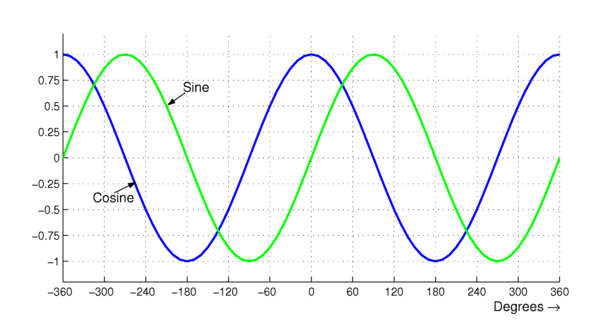
\includegraphics[scale=2]{./diagrams/sinecosine.png}
  \end{figure}
\end{frame}

\begin{frame}
  \frametitle{Trigonometric Functions Review}
  The graph of the tangent functions looks approximately like
  this,
\begin{equation}
  \label{eq:bebiefee}
  \tan\alpha=\frac{\sin\alpha}{\cos\alpha}
\end{equation}
  \begin{figure}[h]
    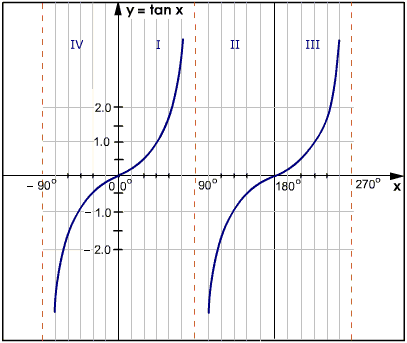
\includegraphics[scale=.5]{./diagrams/tangent.png}
  \end{figure}
\end{frame}

\begin{frame}
  \frametitle{Trigonometric Functions Review}
  Consider the following table of well-known inverse functions
  commonly used in calculus:
  \begin{tabular}{|r|r|}\hline
    \textbf{function} & \textbf{inverse} \\ \hline
    $e^{x}$ & $\ln{}x$ \\ \hline
    $\sin{}x$ & $\arcsin{}x\mbox{ or }\sin^{-1}$ \\ \hline
    $\cos{}x$ & $\arccos{}x\mbox{ or }\cos^{-1}$ \\ \hline
    $\tan{}x$ & $\arctan{}x\mbox{ or }\tan^{-1}$ \\ \hline
  \end{tabular}
\end{frame}

\begin{frame}
  \frametitle{Trigonometric Functions Review}
  Consider the following most important trigonometric identities:
  \begin{equation}
    \label{eq:shutooth}
    \sin{}x^{2}+\cos{}x^{2}=1
  \end{equation}
\begin{equation}
  \label{eq:iegaexah}
  \sin(-\alpha)=-\sin\alpha
\end{equation}
\begin{equation}
  \label{eq:gaijohra}
  \cos(-\alpha)=\cos\alpha
\end{equation}
\begin{equation}
  \label{eq:doajeigh}
  \tan(-\alpha)=-\tan\alpha
\end{equation}
\end{frame}

\begin{frame}
  \frametitle{Trigonometric Functions Review}
  Consider the following most important trigonometric identities:
\begin{equation}
  \label{eq:dieteipa}
  \sin(90^{\circ}-\alpha)=\cos\alpha
\end{equation}
\begin{equation}
  \label{eq:oepoodoh}
  \cos(90^{\circ}-\alpha)=\sin\alpha
\end{equation}
\begin{equation}
  \label{eq:aiwatong}
  \tan(90^{\circ}-\alpha)=\cot\alpha
\end{equation}
\begin{equation}
  \label{eq:jahpeexu}
  \sin(\alpha+180^{\circ})=-\sin\alpha
\end{equation}
\begin{equation}
  \label{eq:aephuemo}
  \cos(\alpha+180^{\circ})=-\cos\alpha
\end{equation}
\begin{equation}
  \label{eq:xaiyahcu}
  \tan(\alpha+180^{\circ})=\tan\alpha
\end{equation}
\begin{equation}
  \label{eq:aitahwae}
  \cot(\alpha+180^{\circ})=\cot\alpha
\end{equation}
\end{frame}

\begin{frame}
  \frametitle{Trigonometric Functions Review}
  Here are the angle sum identities,
  \begin{equation}
  \label{eq:eitaiquu}
  \sin(\alpha+\beta)=\sin\alpha\cos\beta+\cos\alpha\sin\beta
\end{equation}
\begin{equation}
  \label{eq:iasoojou}
  \cos(\alpha+\beta)=\cos\alpha\cos\beta-\sin\alpha\sin\beta
\end{equation}
from which we have, immediately following, the double angle
identities,
  \begin{equation}
    \label{eq:icuchodo}
    \sin(2\alpha)=2\cos\alpha\sin\alpha
  \end{equation}
  \begin{equation}
    \label{eq:woojahtu}
    \cos(2\alpha)=\cos^{2}\alpha-\sin^{2}\alpha
  \end{equation}
\end{frame}

\begin{frame}
  \frametitle{Derivative of Sine}
  The derivative of $f(x)=\sin{}x$ is 
\begin{equation}
  \label{eq:eishooro}
  f'(x)=\lim_{h\rightarrow{}0}\frac{f(x+h)-f(x)}{h}=\lim_{h\rightarrow{}0}\frac{\sin(x+h)-\sin{}x}{h}=\notag
\end{equation}
\begin{equation}
  \label{eq:phauzelo}
  \lim_{h\rightarrow{}0}\frac{\sin{}x\cos{}h+\cos{}x\sin{}h-\sin{}x}{h}=\notag
\end{equation}
\begin{equation}
  \label{eq:jiexeedo}
  \lim_{h\rightarrow{}0}\left[\sin{}x\left(\frac{\cos{}h-1}{h}\right)+\cos{}x\left(\frac{\sin{}h}{h}\right)\right]=\cos{}x
\end{equation}
\end{frame}

\begin{frame}
  \frametitle{The Derivative of Cosine}
The derivative of $f(\vartheta)=\cos\vartheta$ is 
\begin{equation}
  \label{eq:ahfiefev}
  f'(\vartheta)=-\sin\vartheta
\end{equation}
The proof is analogous to the proof for $\sin{}\vartheta$.

\emph{Exercise:} Differentiate 
\begin{equation}
  \label{eq:afeizeix}
  f(t)=\frac{1+\sin{}t}{t+\cos{}t}
\end{equation}
\end{frame}

\begin{frame}
  \frametitle{The Derivative of Tangent}
The derivative of $f(\vartheta)=\tan\vartheta$ is 
\begin{equation}
  \label{eq:uulohjeo}
  f'(\vartheta)=\sec^{2}\vartheta
\end{equation}
Use the quotient rule to prove this. Remember that 
\begin{equation}
  \label{eq:shooceid}
  \sec\vartheta=\frac{1}{\cos\vartheta}
\end{equation}
\end{frame}

\begin{frame}
  \frametitle{Derivatives of Trigonometric Functions}
\begin{figure}[h]
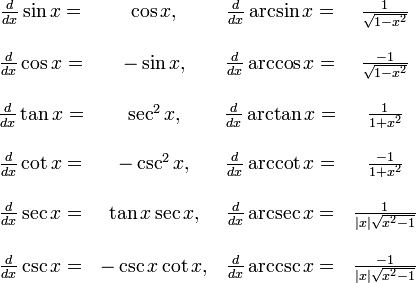
\includegraphics[scale=.6]{./diagrams/trigdiff.png}
\end{figure}
\end{frame}

\begin{frame}
  \frametitle{Exercises}
Differentiate the following functions:
\begin{equation}
  \label{eq:hupuxahz}
  f(x)=3x^{2}-2\cos{}x
\end{equation}
\begin{equation}
  \label{eq:vithooke}
  f(x)=\sqrt{x}\sin{}x
\end{equation}
\begin{equation}
  \label{eq:chaequin}
  f(x)=2\csc{}x+5\cos{}x
\end{equation}
\begin{equation}
  \label{eq:hohxenoo}
  g(t)=4\sec{}t+\tan{}t
\end{equation}
\begin{equation}
  \label{eq:tohsohgh}
  v(w)=\frac{\sin{}w}{w^{2}}
\end{equation}
\begin{equation}
  \label{eq:zichoope}
  f(x)=\csc{}x(x+\cot{}x)
\end{equation}
Find the equation of the tangent line at $(\pi/3,2)$ for
\begin{equation}
  \label{eq:hoirohfo}
  y=\sec{}x
\end{equation}
\end{frame}

\begin{frame}
  \frametitle{End of Lesson}
Next Lesson: Chain Rule
\end{frame}

\end{document}
